\documentclass[28pt,a4paper]{article}
\usepackage[utf8]{inputenc}
\usepackage{lipsum}
\usepackage{color}
\usepackage{amsmath}
\usepackage{multirow}
\usepackage{multicol}
\usepackage{graphicx}
\usepackage{biblatex}
\usepackage{subfigure}
\usepackage{subcaption}
\addbibresource{book.bib}
\title{CSE 300 - Class 1}
\author{Shehabul Islam Sawraz }
\date{\today}

\begin{document}
\maketitle

\tableofcontents %this command creates the table of contents with all numbered sections, subsections, etc.
\pagebreak %This will force the rest of the document to start in another page.

\section{Introduction}
This is a \textbf{bold} text. This is \textit{italic}.

%\lipsum[]

Hey there.\\How are you!!!\par


I am fine...
\paragraph{Bhalo thako \LaTeX!!}

\section{Experiment}\label{sec:exp}
\subsection{Part 1}
\subsection{Part 2}
\subsubsection{Part 2.1}
\subsubsection*{Part 2.2}
\emph{Bhai re bhai!!}\\
{\color{red} Ki r bolbo!! }\\

$a^3+b^3>c^3$

$a^3+b^3 \leq c^3$

$\frac{3}{8}$

This $n$ should be greater than 100

\begin{equation}
    E = mc^2
\end{equation}

\begin{equation}
    y=\sqrt[3]{\frac{x^3}{k+1}}
\end{equation}

\begin{equation}
    \sum_{i=0}^n=x+y
\end{equation}

\begin{equation}
    p(\theta) = \sum_{i=0}^k \phi_i \mathcal{N}(\mu_i,\sigma_i)
\end{equation}

\begin{equation}\label{eqn:normal}
    \mathcal{N}(x_i;\mu, \sigma) = \frac{1}{2\sqrt{\pi}\sigma}e^{-\frac{(x-\mu)^2}{2\sigma^2}}
\end{equation}

Look at equation~\eqref{eqn:normal}\\

\begin{equation}
    |x| =
    \begin{cases}
    \ x & \text{if } x \geq 0 \\
    -x & \text{if } x < 0 \\
    \end{cases}
\end{equation} \\

\begin{align}
    f(x)
    & = (x-1)(x+1) \nonumber\\
    & \qquad +e^x \nonumber\\
    & = x^2 -1 + e^x
\end{align}

\& \\

\section{Table}

\begin{tabular}{|c | c | c | c|}
    \hline
     1&2&3&4  \\
     \hline
     \multicolumn{2}{c|}{\multirow{2}{*}{text}}&6&7 \\ 
     %\hline
     \cline{3-4}
     \multicolumn{2}{|c|}{}&6&7 \\ 
     \hline
\end{tabular}\\

\subsection{Basic Table}
\begin{tabular}{|c|c|c|c|}
    \hline
    \multicolumn{1}{|r|}{1}&2&3&4\\
    \cline{1-3}
    %\hline
    1&2&3&4\\
    \hline
    \multicolumn{3}{|c|}{text} & 4\\
    \hline
    \multirow{2}{*}{text} &2&3&4\\
    \cline{2-4}
    &2&3&4\\
    \hline
    \multicolumn{3}{|c|}{\multirow{2}{*}{text}} &5\\
    \multicolumn{3}{|c|}{}&7\\
    \hline
\end{tabular}\\

\subsection{Table 1}

\begin{tabular}{|c| c cc|}
    \hline
    1&2&3&4\\
    \cline{1-3}
    1&2&3&4\\
    \hline
\end{tabular}\\

\subsection{Table 2}

\begin{tabular}{|c|c c c|}
     \hline
     1 & \multicolumn{3}{|c|}{text}\\
     \cline{2-4}
     1&2&3&4\\
     \hline
\end{tabular}\\

\subsection{Table 3}
\begin{tabular}{|c p{2cm}|}
    \hline
    x & y (in centimeter) \\
    \hline
    1 & \multicolumn{1}{r|}{2} \\
    200 & 400 \\
    \hline
\end{tabular}\\

\textbf{\textit{BOLD & ITALIC}}

\subsection{Table}
\begin{table}[tbp]
    \centering
    \begin{tabular}{|c c|}
        \hline
        x & y \\
        \hline
        1 & 2 \\
        200 & 400 \\
        \hline
    \end{tabular}
    \caption{New Table}
    \label{tab:my_label}
\end{table}

\begin{figure}[htpb] % h means here, t hoile top bujhaito, b mane before bottom, p mane jei page e lekhsi tar porer page e boshanor try korbe, kono option na dile top e try korbe, !h dile gurantee korbe j eikhanei bujhabe onnano jinish k block kore
    \centering
    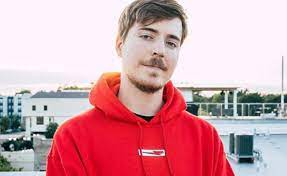
\includegraphics[width=\textwidth]{mrbeast.jpg}
    \caption{Mr Beast}
    \label{fig:beast}
\end{figure}

\begin{figure}[htpb] % h means here, t hoile top bujhaito, b mane before bottom, p mane jei page e lekhsi tar porer page e boshanor try korbe, kono option na dile top e try korbe, !h dile gurantee korbe j eikhanei bujhabe onnano jinish k block kore
    \centering
    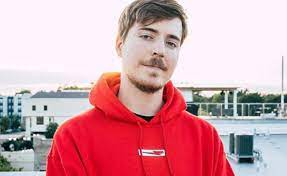
\includegraphics{mrbeast.jpg}
    \caption{Mr Beast}
    \label{fig:beast}
\end{figure}

Above in figure \ref{fig:beast}, we see a youtuber who is poor!!
In section \ref{sec:exp}, its time for experiment brooosss!!

\begin{itemize}
    \item Nafee
    \item Mobs
    \begin{enumerate}
        \item Ami
        \item Redwan
    \end{enumerate}
\end{itemize}

In this course we are citing:
\cite{book1}
\cite{book2}

\begin{figure}
    \centering
    \begin{subfigure}[b]{width=0.15\textwidth}
    \centering
    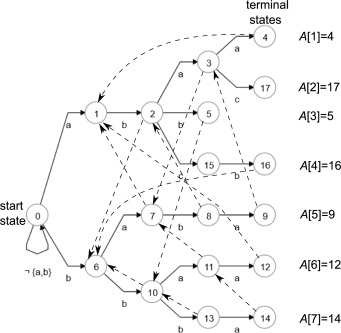
\includegraphics[width=0.15\textwidth]{img.jpg}
    \caption{Pic 1}
    \end{subfigure}
    
    \begin{subfigure}[b]{width=0.15\textwidth}
    \centering
    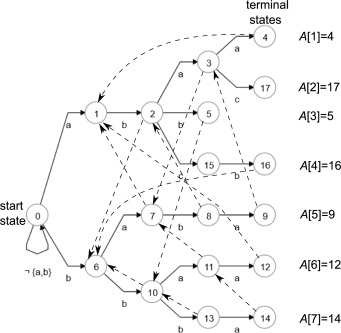
\includegraphics[width=0.15\textwidth]{img.jpg}
    \caption{Pic 2}
    \end{subfigure}
    
    \begin{subfigure}[b]{width=0.15\textwidth}
    \centering
    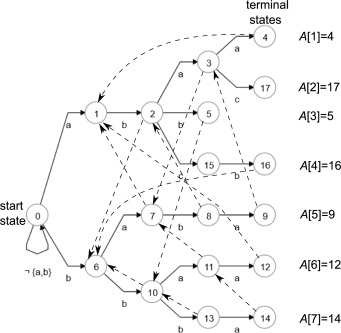
\includegraphics[width=0.15\textwidth]{img.jpg}
    \caption{Pic 3}
    \end{subfigure}
    
    \caption{Caption}
    \label{fig:my_label}
\end{figure}



\printbibliography
\end{document}
